% Klassifiziert den Dokumenten-Typ
% Doku: http://exp1.fkp.physik.tu-darmstadt.de/tuddesign/
% Farben: http://www.tu-darmstadt.de/media/medien_stabsstelle_km/services/medien_cd/das_bild_der_tu_darmstadt.pdf
%  bigchapter: Chapter haben doppelte Schriftgröße
%  linedtoc: Linien im Inhaltsverzeichnis wie bei Überschriften
%  colorbacktitle: Der Dokumenten-Titel wird mir der Accentfarbe hinterlegt
\documentclass[bigchapter,colorback,accentcolor=tud4b,linedtoc,11pt]{tudreport}

% Input Dokument hat das Encoding UTF-8
\usepackage[utf8]{inputenc}
% Wichtiges Paket für Links und verlinktes Inhaltsverzeichnis
\usepackage[ngerman]{hyperref}
% Paket für Fußnoten
\usepackage[stable]{footmisc}
% Paket für amsmath (aligned mathe formeln)
\usepackage{amsmath}
% Paket für Bibliotheks-Verzeichnis, square: Verwende eckige statt runde klammern
% \usepackage[square]{natbib}
% Paket zum Plotten von Datensätzen
\usepackage{pgfplots}
\pgfkeys{
  /pgfplots/PolarStyle/.style={
    ylabel=Leistung in W,
    width=0.33\linewidth,
    height=0.33\linewidth,
    scale only axis,
    grid=both,
    tick align=outside,
    tickpos=left,
    minor x tick num=2,
    minor y tick num=1
  }
}

\usetikzlibrary{pgfplots.polar}
% Verwende deutsche Bezeichner für Inhaltsverzeichnis, ... (ngerman = New German: neue Rechtschreibung)
\usepackage{ngerman}
% Deutsche Zahlen (entfernt z.B. das Leerzeichen nach einem Dezimal-Komma)
\usepackage{ziffer} 

\usepackage[verbose]{placeins}

%wegen Grafikverschiebung hinzugefügt
\usepackage{float}

%\usepackage{graphicx}
%\usepackage{caption}
\usepackage{subcaption} %Für subfigures

% PDF-Optionen
\hypersetup{
  pdftitle={TU Darmstadt \- Physikalisches Praktikum für Fortgeschrittene},
  pdfauthor={Esra Bauer und Sören Link},
  pdfsubject={Versuch 3.3-B},
  pdfview=FitH,
}
% Nummeriere formeln in Subsections einzeln
% Kleines makro zur assymetrischen Fehlerangabe

% Entspricht-Zeichen
\usepackage{scalerel}

\newcommand\equalhat{%
\let\savearraystretch\arraystretch
\renewcommand\arraystretch{0.3}
\begin{array}{c}
\stretchto{
    \scalerel*[\widthof{=}]{\wedge}
    {\rule{1ex}{3ex}}%
}{0.5ex}\\ 
=%
\end{array}
\let\arraystretch\savearraystretch
}
%BEGINN TITELSEITE

\title{Polarisationsanalyse von Licht mittels Stokes-Formalismus}

\subtitle{Esra Bauer  \\Sören Link}

\subsubtitle{Betreuer: David Rupp \hfill Versuchsdatum: 10. November 2014}

\author{Esra Bauer, Sören Link}

%\settitlepicture{img/title.jpg}

\institution{Physikalisches Praktikum \\für Fortgeschrittene \\ Versuch 3.3-B}

\date{\today}


%ENDE TITELSEITE

\begin{document}
%ANFANG DOKUMENT

%Titelseite einfügen
\maketitle

%Inhaltsverzeichnis einfügen
\tableofcontents

%ANFANG INHALT

\chapter{Einleitung}

In diesem Versuch wird Licht verschiedener Polarisationszustände hergestellt und untersucht mit dem Ziel, diese Zustände anschließend vollständig beschreiben zu können, das heißt sowohl für vollständig als auch für teilweise polarisiertes Licht. Wenn man von polarisiertem Licht spricht, bezieht man sich stets auf die Richtung, in der der elektrische Feldvektor oszilliert. Wir betrachten im Folgenden Licht im kartesischen Koordinatensystem, also eine transversale elektromagnetische Welle, welche sich in z-Richtung ausbreitet. Zur Einordnung der Polarisation ist folglich das Verhalten der Elektrischen Feldkomponenten $E_x$ und $E_y$ von Bedeutung.

\chapter{Grundlagen}
\section{Polarisation}

Bei unpolarisiertem Licht, beispielsweise dem Licht der Sonne oder eine Glühlampe, existiert keine feste Beziehung zwischen den Feldkomponenten $E_x$ und $E_y$ bezüglich der Phasenverschiebung $\delta$ und der Beträge $E_{i}$. Schwingt der Feldvektor in einer Ebene, das heißt gilt $\delta=0$, liegt lineare Polarisation vor. Rotiert der Feldvektor um die z-Achse, liegen eine Phasenverschiebung $\delta=\frac{\pi}{2}$ und $E_{x}=E_{y}$ zu Grunde und man spricht von zirkular polarisiertem Licht. Falls $\delta$ einen anderen, jedoch festen Wert annimmt und $E_{x}\neq E_{y}$ gilt, ist die Polarisation elliptisch. 


\section{Stokes-Formalismus}

Mittels des sogenannten Stokes-Formalismus wird es möglich, Mischformen der Polarisationszustände zu klassifizieren und auch den Grad der Polarisation zu bestimmen. Dazu werden die vier Stokes-Parameter wie folgt definiert:

\begin{align*}
  S_0 &= P_{0} + P_{90} = E_{0x}^2 + E_{0y}^2,\\
  S_1 &= P_{0} - P_{90} = E_{0x}^2 - E_{0y}^2,\\
  S_2 &= P_{45} - P_{135} = 2E_{0x} \cdot E_{0y} \cdot cos(\delta),\\
  S_3 &= P_{rechts} - P_{links} = 2E_{0x} \cdot E_{0y} \cdot sin(\delta)
\end{align*}

Das Heißt $S_0$ gibt die Gesamtintensität an, während $S_1$ den in x- oder y- Richtung linar polarisierten Anteil angibt, $S_2$ den Anteil zur x- oder y Achse um 45° Grad verdreht und $S_3$ den rechts- beziehungsweise links zirkular polarisierten Anteil. Wir schreiben die Parameter als Spaktenvektor, den sogenannten Stokes-Vektor $S$, da es sich herausgestellt hat, dass aus einzelnen Stokes-Vektoren durch vektorielle Addition sinnvolle resultierende Stokes-Vektoren ergeben, auch wenn der Stokes-Vektor im streng mathematischen Sinn kein Vektor ist.
Es geht also bei diesem Versuch im Wesentlichen darum, für verschiedene Lichtquellen unbekannter Polarisation die entsprechenden Stokes-Vektoren zu berechnen und somit die Polarisation zu bestimmen. Dazu ist es nötig, sich zunächst mit den verwendeten Lichtquellen und der Erzeugung von Polarisation zu befassen. Im Versuch werden eine weiße LED und ein oberflächenemittierender Halbleiterlaser als Lichtquelle verwendet. 


\section{Lichtemittierende Dioden und Halbleiterlaser}

Beide Lichtquellen senden Licht nach dem Prinzip von p-n-Übergängen aus, das heißt ein p-dotierter Halbleiter, dessen Ladungsträger "Löcher" sind und ein n-dotierter Halbleiter, dessen Ladungsträger Elektronen sind, stehen in Kontakt, wodurch sich eine sog. Verarmungs- bzw. Raumladungszone ausbildet, das heißt an der Kontaktstelle rekombinieren Elektronen und Löcher derart, dass sich die Fermi-Energien der beiden Materialien angleichen. Nun wird eine Spannung von außen in Durchlassrichtung angelegt, wodurch zusätzliche Elektronen in die n-dotierte Schicht eingebracht werden und zur Verarmungszone wandern, wo sie mit Löchern der p-dotierten Schicht rekombinieren und dabei Energie in Form von Licht freisetzen. Die Wellenlänge ist durch die Größe der Bandlücke bestimmt, da der Energiebetrag der Größe der Bandlücke entspricht. Das heißt derartige Lichtquellen senden im Wesentlichen monochromatisches Licht aus und um die besagte weiße LED realisieren zu können, müssen entweder mehrere Halbleiderdioden verschiedener Farben kombiniert werden oder Lumineszenzfarbstoffe auf eine blaue LED aufgebracht werden. Ein weiterer Unterschied zwischen der weißen LED und dem Laser ist der optische Resonator, den nur der Laser besitzt. Im Falle des oberflächenemittierenden Lasers ist der Resonator vertikal ausgerichtet und besteht aus zwei DBR-Spiegeln (engl.: Distributed Bragg Reflectors), zwischen denen konstruktive Interferenz stattfindet. Der Resonator ist extrem kurz (in der Größenordnung einer Wellenlänge), wodurch die Besetzungsinversion, die für das Laserprinzip erforderlich ist, bereits bei einem sehr niedrigem Schwellstrom entsteht.

\section{Polarisatoren und $\frac{\lambda}{4}$-Plättchen}
Beiden Lichtquellen ist gemeinsam, dass sie keine stabile Polarisation besitzen, das heißt diese muss im Versuch selbst hergestellt werden. Zu diesem Zweck bedienen wir uns des Prinzips der Doppelbrechung. Dabei wird Licht, wenn es auf ein doppelbrechendes Material trifft, in zwei Teilstrahlen aufgespalten, für die unterschiedliche Brechungsindizes gelten. Man unterscheidet den ordentlichen Strahl, dessen Polarisation linear und senkrecht zur optischen Achse des Materials (i.d.R. ein Kristall wie z.B. Calcit) ist und der dem Snellius'schen Brechungsgesetz genügt, und den außerordentlichen Strahl, der parallel zur optischen Achse polarisiert ist und dessen Brechungsindex von der Ausbreitungsrichtung relativ zur optischen Achse abhängt. Das Heißt auf diese Weise können wir linear polarisiertes Licht erzeugen. Im Speziellen arbeiten wir mit Glan-Thomson-Polarisationsprismen, die aus zwei Prismen aus doppelbrechendem Material derart zu einen Quader verbunden sind, dass die opische Achse parallel zur Eintrittsfläche liegt und der ordentliche Strahl an der schrägen Verbindungsfläche beider Prismen total reflektiert wird. Der außerordentliche Strahl tritt ohne Ablenkung wieder aus und ist nun linear polarisiert.

\vspace{\baselineskip}Um zirkular polarisiertes Licht zu erzeugen, wird linear polarisiertes Licht auf ein $\frac{\lambda}{4}$-Plättchen gestrahlt. Dieses besteht wieder aus einem doppelbrechenden Material, dessen optische Achse senkrecht zur Ausbreitungsrichtung steht. Beide Teilstrahlen, ordentlicher und außerordentlicher Strahl treten in gleicher Richtung wieder aus, jedoch mit einer Phasendifferenz von $\frac{\pi}{2}$, das heißt es entsteht zirkular polarisiertes Licht. Im Versuch werden sogenannte zusammengesetzte $\frac{\lambda}{4}$-Plättchen nullter Ordnung verwendet, das heißt das Licht strahlt durch zwei doppelbrechende Materialen, deren optische Achsen senkrecht zueinander ausgerichtet sind. Die Phasenverschiebung kommt nicht durch die Gesamtdicke des Plättchens zustande, sondern durch die Dickendifferenz der beiden Bestandteile. Dieser Trick ist notwendig, da sich solch geringe Dicken, wie sie für Licht notwendig wären, nicht ohne weiteres herstellen und händeln lassen. Es ist zu beachten, dass das $\frac{\lambda}{4}$-Plättchen tatsächlich nicht genau um $\frac{\pi}{2}$ verzögert, sondern je nach Wellenlänge eine mehr oder weniger starke Abweichung besteht. Um dies im Verlauf des Versuchs zu untersuchen, benötigen wir einen Babinet-Soleil-Kompensator (im Folgen als BSK bezeichnet). Es handelt sich dabei grundsätzlich um ein verstellbares zusammengesetztes Verzögerungsplättchen nullter Ordnung, d.h. wie auch bei den verwendeten $\frac{\lambda}{4}$-Plättchen liegen zwei doppelbrechende Materialien derart aufeinander, dass die optischen Achsen senkrecht zueinander sind. Jedoch besteht beim BSK eine der Platten aus zwei Keilen, die per Stellschraube gegeneinander verschoben werden können, wodurch sich die Dickendifferenz und somit die Phasenverschiebung ändert. 

\section{Müller-Matrix-Formalismus}
Wie oben beschrieben, lassen sich mit Stokes Vektoren $\vec{S}= (S_0, S_1, S_2, S_3)^T$ resultierende Polarisationszustände berechnen. Das legt nahe, dass man auch Matrizen auf diese Vektoren anwenden darf. Man kann in der Tat optischen Bauteilen sog. Müller-Matrizen zuordnen, die als Transformationsmatrizen für die Stokes Vektoren dienen. Ist ein einfallender Lichtstrahl durch den Stokes-Vektor $S$ charakterisiert und ein optisches Bauteil durch die Müller-Matrix $M$, so ergibt sich der austretende Lichtstrahl zu $S' = M \cdot S$ 

\section{Drehwinkelaufnehmer}
Um die Winkelposition eines $\frac{\lambda}{4}$-Plättchens oder eines Polarisators kontrollieren zu können bzw. Kennlinien über dem Drehwinkel aufnehmen zu können, stehen uns Drehwinkelaufnehmer, in die jeweils ein $\frac{\lambda}{4}$-Plättchen und ein Polarisator eingebaut ist, zur Verfügung. Damit ist es uns möglich, den Winkel in Schritten von 5 Grad aufzunehmen, da auf der Oberfläche des Drehwinkelaufnehmers stark und schwach reflektierende Beschichtungen abwechselnd (in 5 Grad Unterteilung) aufgebracht sind, die von einer Reflexionslichtschranke als Signal verarbeitet werden. Die verwendete Software nimmt automatisch einen Leistungswert vom Detektor auf, sobald ein Signal der Lichtschranke vorliegt. 


\section{Gefahren durch Laserstrahlung und Vorsichtsmaßnahmen}
Bei dem in diesem Versuch vorliegenden VCSEL Laser mit einigen mW Leistung im roten Spektralbereich sind die potentiellen Gefahren durch Laserstrahlung überschaubar. Vor allem muss hier darauf geachtet werden, dass der Laser nicht in ein Auge gelangt. Aus diesem Grund ist bei eingeschaltetem Laser immer eine Schutzbrille zu Tragen und der Kopf ist nie auf Höhe des Lasers zu halten. Auch sollte darauf geachtet werden, dass potentielle Reflexe des Lasers wenn möglich auf die Laserapparatur selbst zurückgelengt werden und vor allem nicht auf einen Eingang zeigen, da sonst außenstehende ohne Schutzbrille gefährdet werden können.

Bei Lasern mit höherer Intensität ist zudem der Kontakt mit dem Körper zu vermeiden, da ein Laser nicht nur oberflächliche Verbrennungen, sondern im Falle eines UV-Lasers auch Hautkrebs und im Falle eines IR-Lasers schmerzlose und deswegen schwer zu erkennende Verbrennungen im Unterhautgewebe verursachen können. Zur Sichtbarmachung von Lasern sollte deswegen nie die nackte Haut sondern eine nicht reflektierende Oberfläche (beispielsweise ein Schirm, der die verwende Laserleistung aushält) verwendet werden.

Abgesehen von den genannte Personenschäden sind bei nicht sachgemäßer Handlung von Lasern mit hoher Intensität auch Schäden am Versuchsaufbau möglich. Verschmutzte Spiegel oder Fenster des Lasermediums können zu extremer Hitzeentwicklung an jeweiligen Material und letztendlich zu dessen Ermattung oder gar Zerstörung führen.
%% quellenangabe
\cite{GefahrenLaser}


\chapter{Durchführung}
\section{Aufnahme der P-I-Kennlinie der LED}
\label{sec:pikennlinie}
Zuerst nehmen wir eine P-I-Kennlinie der weißen LED auf. Das heißt, wir messen die abgestrahlte Lichtleistung über dem Strom. Da die LED in einem sehr großen Winkel abstrahlt, verwenden wir hierfür zwei Linsen, um eine Kollimation zu erreichen. Unser Aufbau besteht hierbei aus der LED, den beiden Linsen und dem Detektor, die in dieser Reihenfolge auf einem Reiter montiert werden.
\begin{figure}[ht!]
\centering
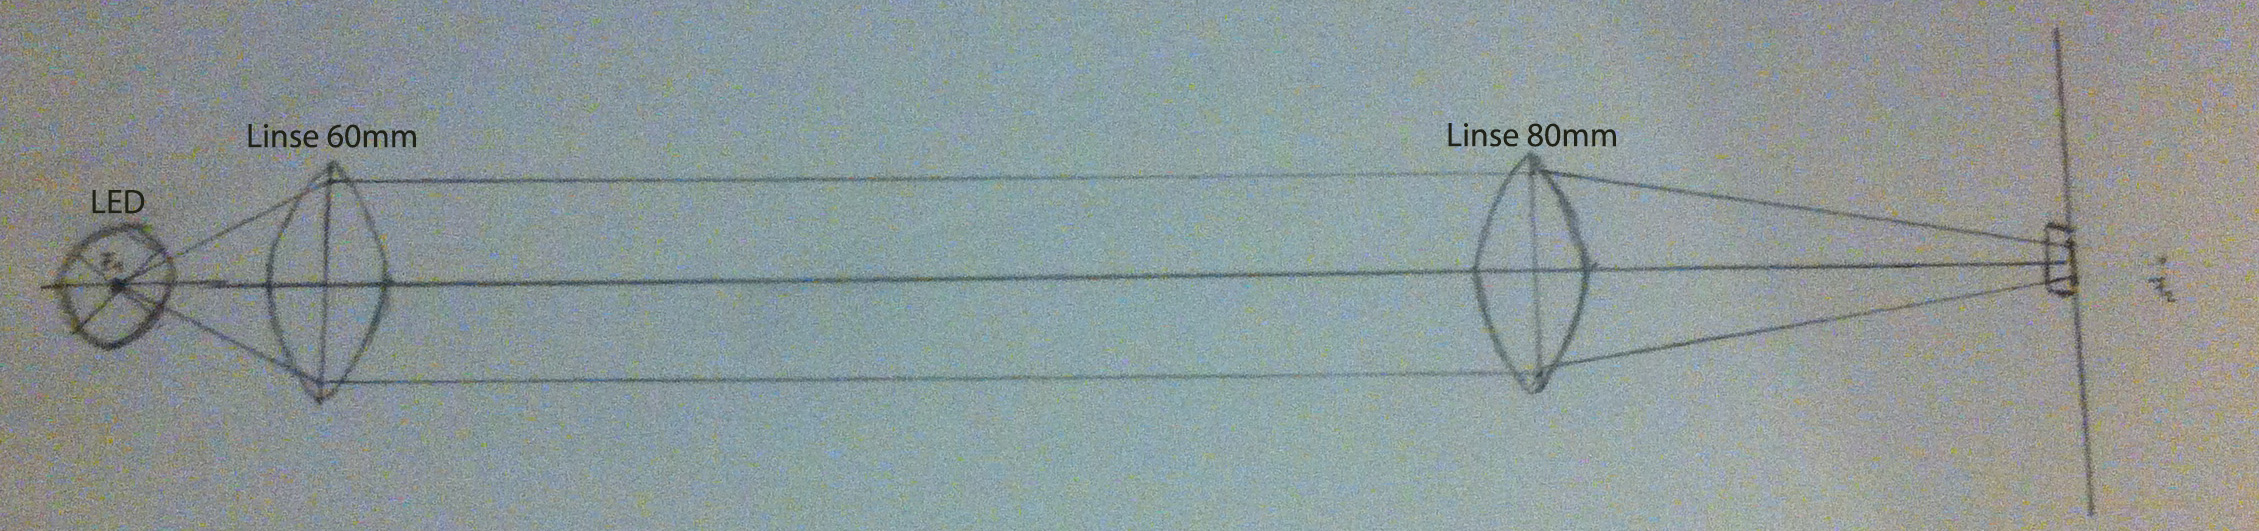
\includegraphics[width=150mm]{img/skizzen/versuch_a.jpg}
\caption{Versuchsaufbau zur Bestiimung der P-I-Kennlinie der LED}
\label{PI-Kennlinie-LED}
\end{figure}
\begin{center}
\begin{figure}[h]
\begin{tikzpicture}
\begin{axis}[
    legend pos=south west,
    title={Leistung der weißen LED in abhängigkeit der Stromstärke},
    xlabel=Stromstärke in mA,
    ylabel=Leistung in W,
    width=0.9\textwidth,
    height= 9cm,
    xmin=0,
    xmax=55,
    grid=both,
    ymin=0,
    ymax=0.0045,
    tick align=outside,
    tickpos=left,
    minor x tick num=3,
    minor y tick num=4,
    minor grid style={dotted,thin}
]
\addplot[red, only marks, mark=x, mark size=1pt, error bars/.cd, y dir=both, y fixed relative=0.01, x dir=both, x fixed=0.05]
table[x index={0},y index={1}] {data/1.txt};
\addlegendentry{Leistung der LED auf der Photoplatte}
\end{axis}
\end{tikzpicture}
\captionof{figure}{Gemessene Leistung der LED auf der Photoplatte in abhängigkeit von der angelegten Stromstärke. Die angenommenen Fehler für die Stromstärke und die gemessene Leistung der LED betragen 0.05mA und 1 Prozent.}
\end{figure}
\end{center}

Als Fehler für die Stromstärke wurden 0.05mA angenommen, da die Stromquelle nur eine Nachkommastelle anzeigte. Dagegen wurde als Fehler für die aufgenommene Leistung 1 Prozent angenommen. Zwar ist das verwendete Messgerät deutlich genauer, allerdings wurden dennoch offensichtliche Schwankungen in der gemessenen Leistung beobachtet, welche entweder durch den im Raum verwendeten Monitor oder durch eine nicht konstante Leistung der LED verursacht wurden.

Bis etwa 20mA nimmt die Leistung der LED angenähert proportional zur angelegten Stromstärke zu, danach scheint sich die Leistung langsam einem Maximalwert anzunähern.

\section{Auslöschungsverhältniss der Linearpolarisatoren}
Zur Bestimmung des Auslöschungsverhältnisses der Linearpolarisatoren wurden in den Aufbau aus Abschnitt~\ref{sec:pikennlinie} noch 2 Linearpolarisatoren eingefügt.
Anschließend wurde einer der Polarisatoren so lange gedreht, bis die aufgenommene Leistung ein Minimum erreicht hat, die Polarisationsachsen der Polarisatoren also um 90° zueinander verdreht waren. Danach wurde der vordere Linearpolarisator um 90° gedreht und es wurde erneut die gemessene Leistung augenommen.

\begin{figure}[ht!]
\centering
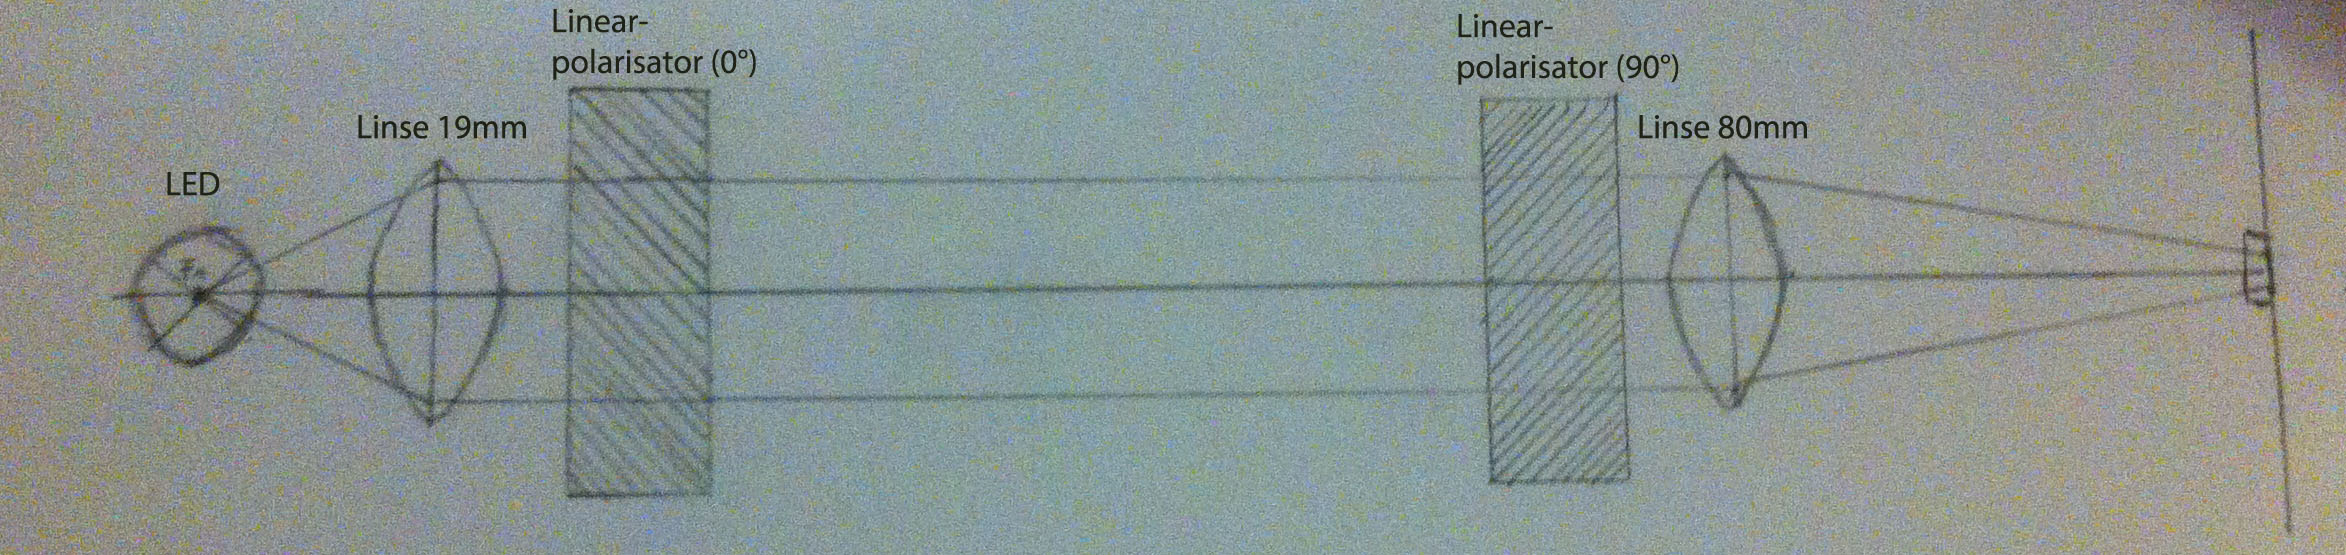
\includegraphics[width=150mm]{img/skizzen/versuch_b.jpg}
\caption{Versuchsaufbau zur Bestimmung des Auslöschungsverhältnisses der Linearpolarisatoren}
\label{Auslöschungsverhältniss-Linearpolarisatoren}
\end{figure}
Folgende Werte wurden aufgenommen:
\begin{center}
  \begin{tabular}{|p{5cm}|p{4cm}|p{4.5cm}|}
    \hline
        Winkel $\alpha$ zwischen den Polarisationsachsen in Grad & Leistung P in W & Fehler $\Delta$P der Leistung in W \\ \hline
        90 & $6,75 \cdot 10^-9$ & $0,05 \cdot 10^-9$ \\ \hline
        0 & $5,111 \cdot 10^-4$ & $0,05 \cdot 10^-4$ \\ \hline
	\end{tabular}
\end{center}
\section{Bestimmung der wellenlängenaufgelösten Verzögerung des achromatischen Verzögerungsplättchens}
Im Abschnitt 2.4 wurde bereits das $\frac{\lambda}{4}$-Plättchen beschrieben. Die schon genannte Wellenlängenabhängigkeit der tatsächlichen Phasenverschiebung soll nun untersucht werden. Zu diesem Zweck verwendenden wir den Babinet-Soleil-Kompensator. 

\begin{figure}[ht!]
\centering
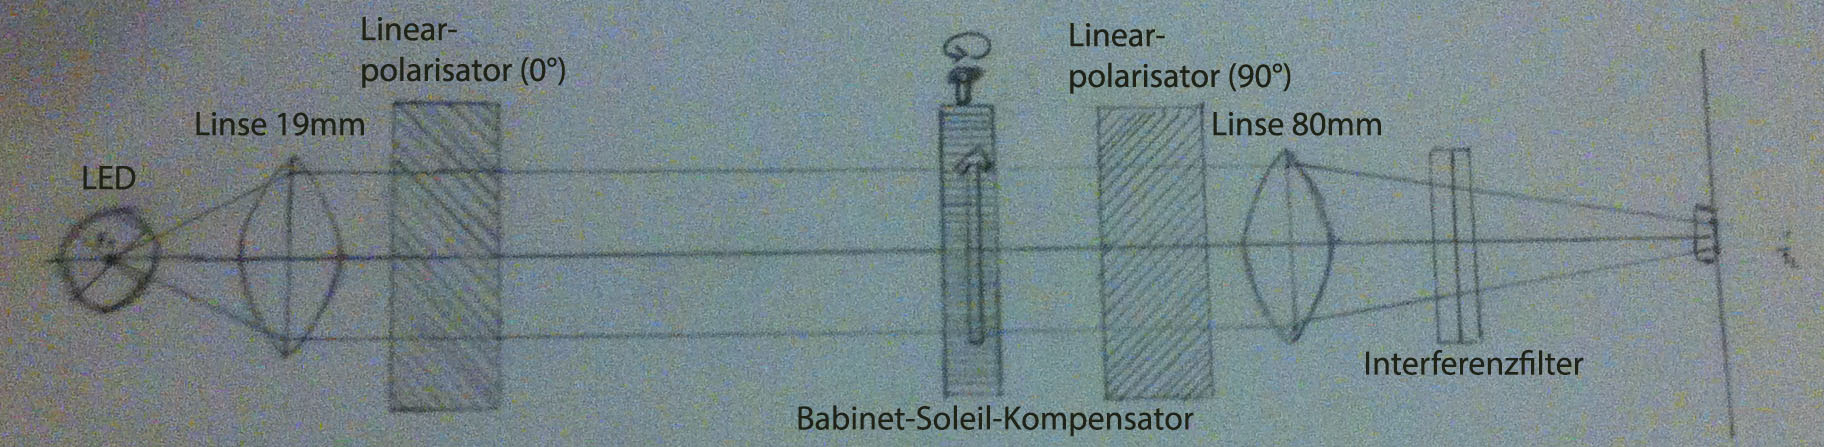
\includegraphics[width=150mm]{img/skizzen/versuch_c_1.jpg}
\caption{Versuchsaufbau zur Kalibration des BSK}
\end{figure}

Da Leistungsminima am einfachsten gemessen werden können, fügen wir den BSK  zwischen beide Polarisatoren ein, die wir vorher senkrecht zueinander ausgerichtet haben (immer in Bezug auf die optischen Achsen) und richten ihn so aus, dass immernoch ein Minimum gemessen wird. Nun verdrehen wir ihn um 45 Grad und justieren die Dicke solange nach, bis drei nebeneinanderliegende Minima gemessen werden können. Diese Messungen führen wir mit verschiedenen Farbfiltern durch, jeweils bei 488nm, 543,5nm, 633nm und 694,3nm, um eine Referenz zu finden.

Bei den verwendeten Farbfiltern handelt es sich um Interferenzfilter, das heißt sie bestehen aus vielen Schichten, die sich in Brechungsindex und Dicke unterscheiden. Das einfallende Licht wird in den jeweiligen Schichten teilweise reflektiert und transmittiert und durch konstruktive und destruktive Interferenz wird erreicht, dass insgesamt lediglich ein schmaler Wellenlängenbereich transmittiert wird. Folgende Werte lesen wir am BSK ab, wobei wir den Fehler mit 0,06 abschätzen: 


\begin{center}
  \begin{tabular}{|c|c|c|c|}
    \hline
        Filter 1 (488nm) & Filter 2 (543,5nm) & Filter 3 (633nm) & Filter 4 (694,3nm) \\ \hline
        30,91 & 29,47 & 27,11 & 25,64 \\ \hline
        42,19 & 42,21 & 42,22 & 42,24 \\ \hline
        53,55 & 54,95 & 57,29 & 58,80 \\ \hline
	\end{tabular}
\end{center}

Anschließend wird das $\frac{\lambda}{4}$-Plättchen in den Strahlengang vor den BSK integriert, nach dem Minimum ausgerichtet, um 45 Grad gedreht und die Messung wiederholt.

\begin{figure}[ht!]
\centering
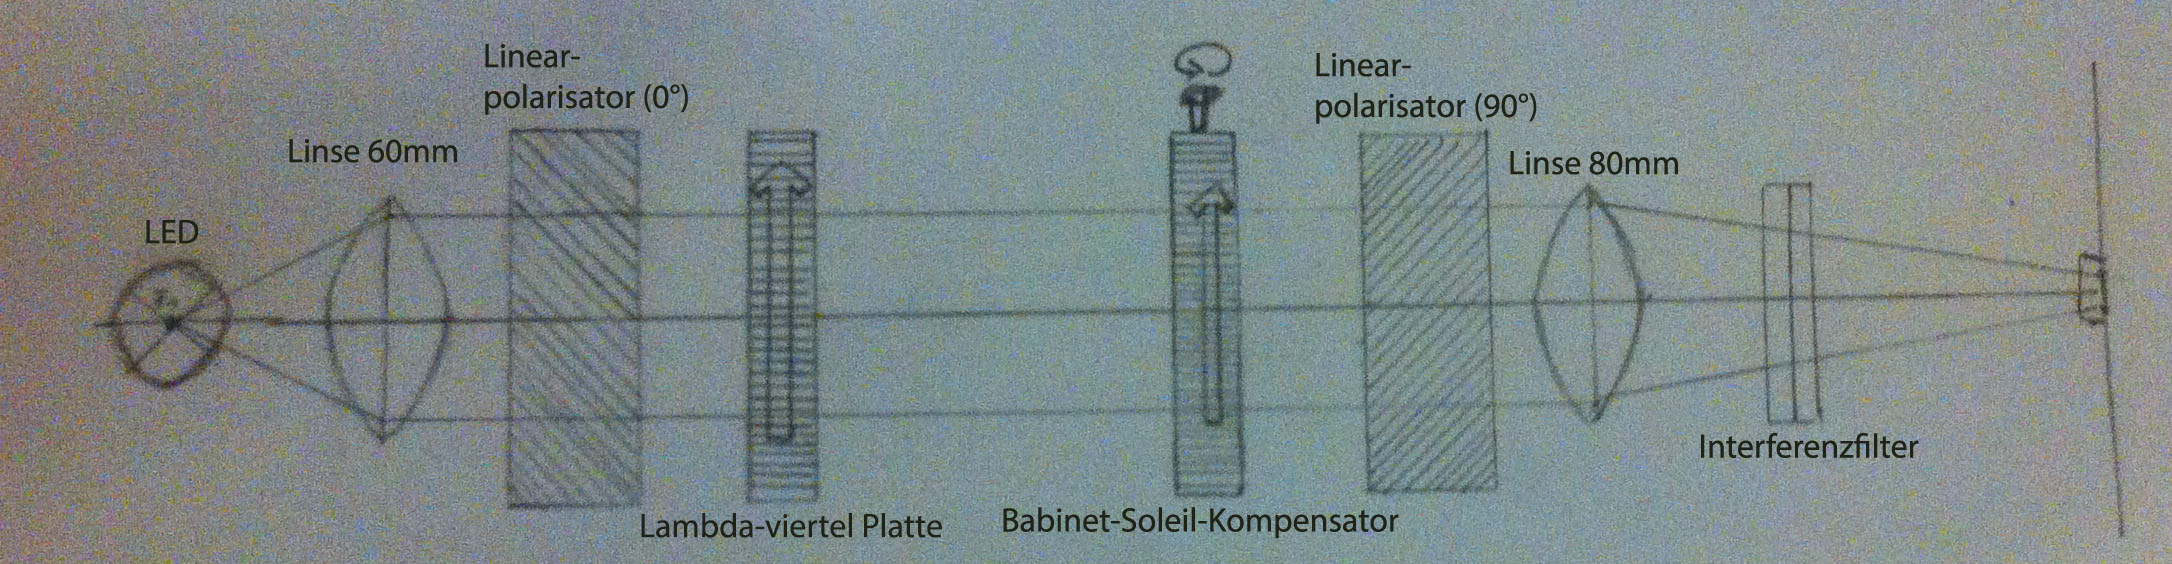
\includegraphics[width=150mm]{img/skizzen/versuch_c_2.jpg}
\caption{Versuchsaufbau zur Bestimmung der genauen Verzögerung des Verzögerungsplättchens}
\end{figure}

Dies liefert uns folgende Werte:

\begin{center}
  \begin{tabular}{|c|c|c|c|}
    \hline
        Filter 1 (488nm) & Filter 2 (543,5nm) & Filter 3 (633nm) & Filter 4 (694,3nm) \\ \hline
        27,97 & 26,18 & 23,41 & 21,60 \\ \hline
        39,33 & 38,95 & 38,48 & 38,22 \\ \hline
        50,62 & 51,67 & 53,50 & 54,81 \\ \hline
	\end{tabular}
\end{center}


Der physikalische Hintergrund dieser Messungen ist, dass wir durch die Einstellung des BSK gerade die Wirkung des Verzögerungsplättchens aufheben, d.h. die Differenzen der am BSK eingestellten Werte mit und ohne  $\frac{\lambda}{4}$-Plättchen ergeben die Phasenverzögerung, wobei wir noch auf ganze Wellenlängen skalieren müssen, also durch 2 dividieren (dies liefert $\delta$ im Bogenmaß) bzw. mit $\frac{360^\circ}{4\pi}$ multiplizieren (damit berechnen wir die Phasenverschiebung im Gradmaß). Die Phasenverschiebungen sind dementsprechend: 

\begin{center}
  \begin{tabular}{|c|c|c|c|}
    \hline
        Filter 1 (488nm) & Filter 2 (543,5nm) & Filter 3 (633nm) & Filter 4 (694,3nm) \\ \hline
        0,468 $\pi$ & 0,524 $\pi$ & 0,589 $\pi$ & 0,643 $\pi$ \\ \hline
        0,455 $\pi$ & 0,519 $\pi$ & 0,595 $\pi$ & 0,640 $\pi$ \\ \hline
        0,466 $\pi$ & 0,522 $\pi$ & 0,603 $\pi$ & 0,635 $\pi$ \\ \hline
	\end{tabular}
\end{center}

Das Messen jeweils dreier Werte ist sinnvoll, um eine größere Genauigkeit zu erreichen. Durch das benutzen von 3 Messdaten kann der erwartete Fehler durch $\sqrt{3}$ geteilt werden.
\section{Charakterisierung des Polarisationszustandes mit Hilfe des Stokes-Formalismus}
Zur Herstellung linearer Polarisation stehen uns die bekannten Glan-Thomson-Polarisationsprismen zur Verfügung. Um daraus zirkular polarisiertes Licht zu erzeugen, bedienen wir uns des $\frac{\lambda}{4}$-Plättchens, dessen Verzögerung wir im vorigen Abschnitt für die jeweiligen Wellenlängen genau bestimmt haben. Im Folgenden werden alle Messungen mit Filter 4 (694,3nm) durchgeführt, das heißt $\delta = (0,639 \pm 9,556 \cdot 10^{-3}) \pi$. Zunächst messen wir ohne $\frac{\lambda}{4}$-Plättchen, richten den 1. Linearpolarisator in y-Richtung aus und nehmen die Leistung über der Winkelposition des zweiten Polarisators auf (wir verwenden also lediglich den Drehwinkelaufnehmer mit Linearpolarisator, der restliche Aufbau bleibt unangetastet). Wir erhalten folgende Verteilung:

\begin{center}
\begin{figure}[H]
\begin{tikzpicture}
\begin{axis}[
    legend pos=south west,
    title={Lichtleistung über dem Drehwinkel},
    xlabel=Drehwinkel in Grad,
    ylabel=Lichtleistung in W,
    width=0.9\textwidth,
    height= 9cm,
    xmin=0,
    xmax=360,
    grid=both,
    ymin=0,
    ymax=0.000007,
    tick align=outside,
    tickpos=left,
    minor x tick num=3,
    minor y tick num=4,
    minor grid style={dotted,thin}
]
\addplot[red, only marks, mark=x, mark size=1pt, error bars/.cd, y dir=both, y fixed relative = 0.01, x dir=both, x fixed = 0]
table[x index={0},y index={1}] {data/d-lin-y.txt};
\addlegendentry{ohne $\frac{\lambda}{4}$-Plättchen}
\end{axis}
\end{tikzpicture}
\captionof{figure}{Linear in y-Richtung polarisiertes Licht}
\end{figure}
\end{center}

Nun wird der Drehwinkelaufnehmer mit $\frac{\lambda}{4}$-Plättchen vor den letzten Polarisator montiert, der 1. Polarisator um 45$^\circ$ gedreht und nun die Lichtleistung über der Winkelposition des $\frac{\lambda}{4}$-Plättchens aufgenommen. 

\begin{center}
\begin{figure}[H]
\begin{tikzpicture}
\begin{axis}[
    legend pos=south west,
    title={Lichtleistung über dem Drehwinkel},
    xlabel=Drehwinkel in Grad,
    ylabel=Lichtleistung in W,
    width=0.9\textwidth,
    height= 9cm,
    xmin=0,
    xmax=360,
    grid=both,
    ymin=0,
    ymax=0.00001,
    tick align=outside,
    tickpos=left,
    minor x tick num=3,
    minor y tick num=4,
    minor grid style={dotted,thin}
]
\addplot[red, only marks, mark=x, mark size=1pt, error bars/.cd, y dir=both, y fixed relative = 0.01, x dir=both, x fixed = 0]
table[x index={0},y index={1}] {data/d-45.txt};
\addlegendentry{mit $\frac{\lambda}{4}$-Plättchen}
\end{axis}
\end{tikzpicture}
\captionof{figure}{+45 Grad}
\end{figure}
\end{center}

Zusätzlich steht uns eine 3D-Kinobrille zur Verfügung, deren optische Eigenschaften genauer untersucht werden sollen. Dazu montieren wir sie auf den Reiter zwischen Linse und Drehwinkelaufnehmer, zunächst so, dass das Licht der LED von innen auf das Brillenglas fällt, das Licht also in Blickrichtung des Brillenträgers propagiert. Wir messen wieder die Lichtleistung über der Winkelposition des Linearpolarisators. 

\begin{center}
\begin{figure}[H]
\begin{tikzpicture}
\begin{axis}[
    legend pos=south west,
    title={Lichtleistung über dem Drehwinkel},
    xlabel=Drehwinkel in Grad,
    ylabel=Lichtleistung in W,
    width=0.9\textwidth,
    height= 8cm,
    xmin=0,
    xmax=360,
    grid=both,
    ymin=0,
    ymax=0.000016,
    tick align=outside,
    tickpos=left,
    minor x tick num=3,
    minor y tick num=4,
    minor grid style={dotted,thin}
]
\addplot[red, only marks, mark=x, mark size=1pt, error bars/.cd, y dir=both, y fixed relative = 0.01, x dir=both, x fixed = 0]
table[x index={0},y index={1}] {data/d-brille-1-licht in sichtrichtung.txt};
%\addlegendentry{}
\end{axis}
\end{tikzpicture}
\captionof{figure}{3D-Kinobrille, Lichtbestrahlung in Blickrichtung des Brillenträgers}
\end{figure}
\end{center}

Nun wiederholen wir dieselbe Messung, jedoch drehen wir die Brille um, so dass das Licht in entgegengesetzer Richtung auf das Brillenglas fällt (entgegen der Blickrichtung des Brillenträgers).

\begin{center}
\begin{figure}[H]
\begin{tikzpicture}
\begin{axis}[
    legend pos=south west,
    title={Lichtleistung über dem Drehwinkel},
    xlabel=Drehwinkel in Grad,
    ylabel=Lichtleistung in W,
    width=0.9\textwidth,
    height= 8cm,
    xmin=0,
    xmax=360,
    grid=both,
    ymin=0,
    ymax=0.000016,
    tick align=outside,
    tickpos=left,
    minor x tick num=3,
    minor y tick num=4,
    minor grid style={dotted,thin}
]
\addplot[red, only marks, mark=x, mark size=1pt, error bars/.cd, y dir=both, y fixed relative = 0.01, x dir=both, x fixed = 0]
table[x index={0},y index={1}] {data/d-brille-2.txt};
%\addlegendentry{}
\end{axis}
\end{tikzpicture}
\captionof{figure}{3D-Kinobrille, Lichtbestrahlung gegen Blickrichtung des Brillenträgers}
\end{figure}
\end{center}

\section{P-I-Kennlinie der VCSEL}
TODO: Skizze
Analog zur Aufnahme der P-I-Kennlinie der LED nehmen wir ebenfalls die P-I-Kennlinie der VCSEL auf. Hierzu wird im Aufbau die LED mit dem VCSEL ausgetauscht und auf diie erste Linse zur Kolimation des Lichts verzichtet, da der VCSEL bereits kolimiertes licht emittiert.
\begin{figure}[ht!]
\centering
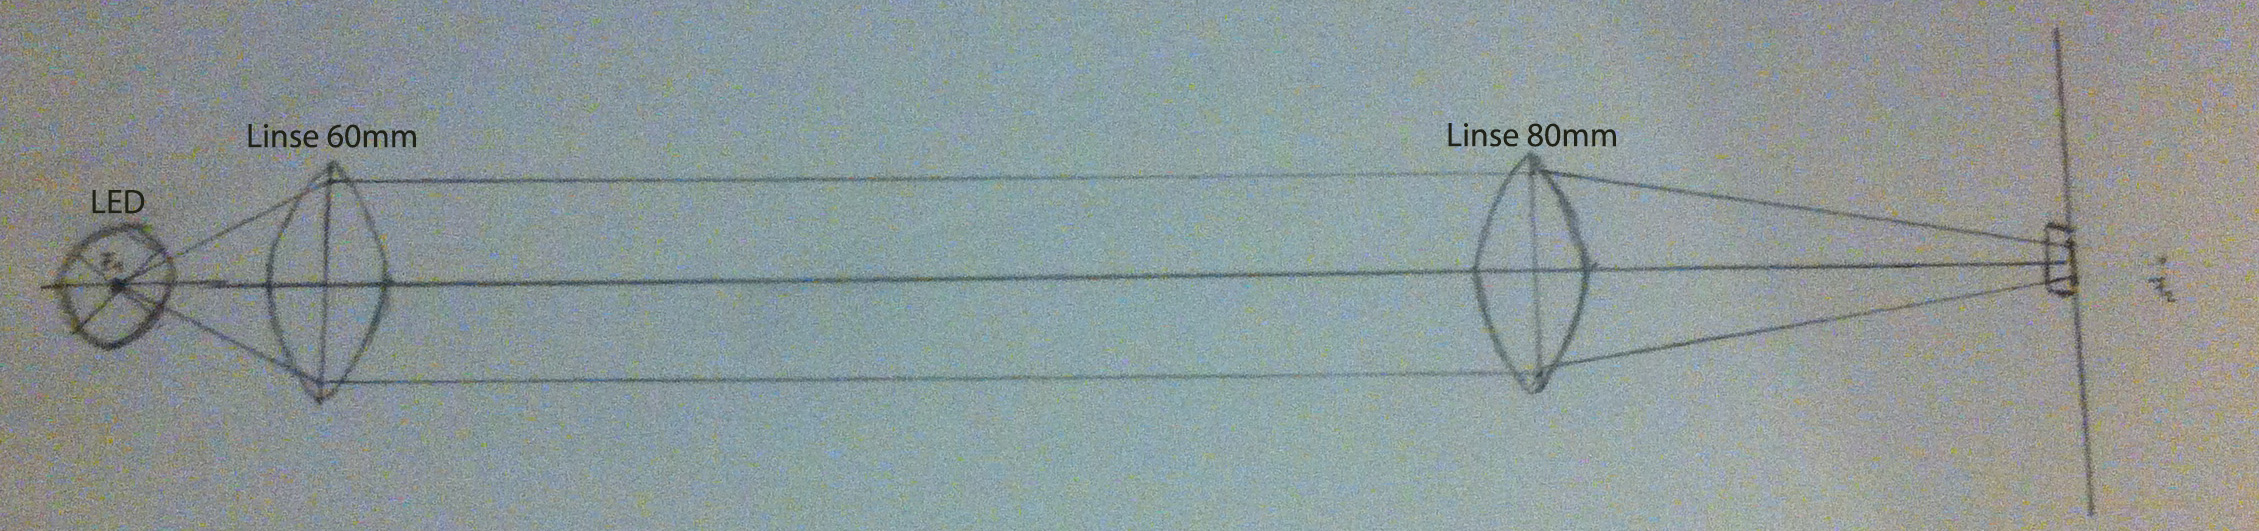
\includegraphics[width=150mm]{img/skizzen/versuch_a.jpg}
\caption{Versuchsaufbau zur Bestiimung der P-I-Kennlinie der VCSEL}
\label{PI-Kennlinie-VCSEL}
\end{figure}

\begin{center}
\begin{figure}[h]
\begin{tikzpicture}
\begin{axis}[
    legend pos=south east,
    title={Leistung der VCSEL in abhängigkeit der Stromstärke},
    xlabel=Stromstärke in mA,
    ylabel=Leistung in W,
    width=0.9\textwidth,
    height= 9cm,
    xmin=0,
    xmax=13,
    grid=both,
    ymin=0,
    ymax=0.0022,
    tick align=outside,
    tickpos=left,
    minor x tick num=3,
    minor y tick num=4,
    minor grid style={dotted,thin}
]
\addplot[red, only marks, mark=x, mark size=1pt, error bars/.cd, y dir=both, y fixed relative=0.01, x dir=both, x fixed=0.05]
table[x index={0},y index={1}] {data/e-P-I.txt};
\addlegendentry{Leistung der VCSEL auf der Photoplatte}
\end{axis}
\end{tikzpicture}
\captionof{figure}{Gemessene Leistung der VCSEL auf der Photoplatte in abhängigkeit von der angelegten Stromstärke. Die angenommenen Fehler für die Stromstärke und die gemessene Leistung der VCSEL betragen 0.05mA und 1 Prozent.}
\end{figure}
\end{center}

Analog zu Abschnitt 3.1 wurde als Fehler für die Stromstärke 0.05mA und als Fehler für die aufgenommene Leistung 1 Prozent angenommen.

\section{Polarisationszustand des VCSELs in Abhägigkeit des Stroms}
VCSEL haben in der regel keine feste Polarisation, vielmehr variirt die Art und der Grad der Polarisation auf grund von thermischer Ausdehnung einzelner Komponenten mit der angelegten Stromstärke. Zur Untersuchung dieser Eigenschaft haben wir die winkelabhängige Leistung des VCSELs mit Hilfe des Drehwinkelaufnehmers bei 3.5mA, 4mA, 6mA, 8mA, 10mA und 12mA bestimmt.

Dazu haben wurde der von der VCSEL emmitierte Strahl zuerst durch einen Linearpolarisator, dann durch den Drehwinkelaufnehmer und anschließend durch einen um 90° verdrehten Linearpolarisator gelenkt.

\begin{figure}[h]
\begin{tikzpicture}
\begin{polaraxis}[
  PolarStyle,
  ymin=-9e-7,
  ymax=9e-7,
  name=first
]
\addplot[red, only marks, mark=x, mark size=2pt]
table[x index=0,y index=1] {data/f-1.txt};
\addlegendentry{1mA}
\end{polaraxis}

\begin{polaraxis}[
  PolarStyle,
  name=second,
  at=(first.outer south east),
  anchor=outer south west
]
\addplot[blue, only marks, mark=x, mark size=2pt]
table[x index=0,y index=1, data cs=polar] {data/f-2.txt};
\addlegendentry{2mA}
\end{polaraxis}

\begin{polaraxis}[
  PolarStyle,
  name=third,
  at=(first.outer south west),
  anchor=outer north west,
  yshift=-0.25cm
]
\addplot[orange, only marks, mark=x, mark size=2pt]
table[x index=0,y index=1, data cs=polar] {data/f-2,5.txt};
\addlegendentry{2,5mA}
\end{polaraxis}

\begin{polaraxis}[
  PolarStyle,
  name=fourth,
  at=(third.outer south east),
  anchor=outer south west
]
\addplot[black, only marks, mark=x, mark size=2pt]
table[x index=0,y index=1, data cs=polar] {data/f-3.txt};
\addlegendentry{3mA}
\end{polaraxis}
\end{tikzpicture}
\captionof{figure}{Leistung in Abhängigkeit der Ausrichtung des Drehwinkelmessers für einen angelegten Strom von 1mA, 2mA, 2,5mA und 3mA. Es ist eindeutig eine Zunahme des Polarisationsgrades des emmitierten Lichtes zu sehen. Bei 3mA ist bereits eine deutliche Polarisation feststellbar}
\end{figure}


\begin{figure}[h]
\begin{tikzpicture}
\begin{polaraxis}[
  PolarStyle,
  name=first
]
\addplot[red, only marks, mark=x, mark size=2pt]
table[x index=0,y index=1, data cs=polar] {data/f-3,5.txt};
\addlegendentry{3.5mA}
\end{polaraxis}

\begin{polaraxis}[
  PolarStyle,
  name=second,
  at=(first.outer south east),
  anchor=outer south west
]
\addplot[blue, only marks, mark=x, mark size=2pt]
table[x index=0,y index=1, data cs=polar] {data/f-4.txt};
\addlegendentry{4mA}
\end{polaraxis}

\begin{polaraxis}[
  PolarStyle,
  name=third,
  at=(first.outer south west),
  anchor=outer north west,
  yshift=-0.25cm
]
\addplot[orange, only marks, mark=x, mark size=2pt]
table[x index=0,y index=1, data cs=polar] {data/f-6.txt};
\addlegendentry{6mA}
\end{polaraxis}

\begin{polaraxis}[
  PolarStyle,
  name=fourth,
  at=(third.outer south east),
  anchor=outer south west
]
\addplot[black, only marks, mark=x, mark size=2pt]
table[x index=0,y index=1, data cs=polar] {data/f-8.txt};
\addlegendentry{8mA}
\end{polaraxis}

\begin{polaraxis}[
  PolarStyle,
  name=fith,
  at=(third.outer south west),
  anchor=outer north west,
  yshift=-0.25cm
]
\addplot[brown, only marks, mark=x, mark size=2pt]
table[x index=0,y index=1, data cs=polar] {data/f-10.txt};
\addlegendentry{10mA}
\end{polaraxis}

\begin{polaraxis}[
  PolarStyle,
  name=sixth,
  at=(fith.outer south east),
  anchor=outer south west
]
\addplot[purple, only marks, mark=x, mark size=2pt]
table[x index=0,y index=1, data cs=polar] {data/f-12.txt};
\addlegendentry{12mA}
\end{polaraxis}
\end{tikzpicture}
\captionof{figure}{Leistung in Abhängigkeit der Ausrichtung des Drehwinkelmessers für einen angelegten Strom von 3.5mA, 4mA, 6mA, 8mA, 10mA und 12mA. Mit bloßem Auge ist hier keine weitere zunahme des Polarisationsgrades mehr zu sehen, es liegt durchgehend zirkular polarisiertes Licht vor.}
\end{figure}


\chapter{Auswertung}
\section{Aufnahme der P-I-Kennlinie der LED}
TODO: Tabelle, Graph, Fehlerrechnung

\section{Auslöschungsverhältniss der Linearpolarisatoren}
Aus den für die beiden Linearpolarisatoren aufgenommenen Werten
\begin{center}
  \begin{tabular}{|p{5cm}|p{4cm}|p{4.5cm}|}
    \hline
        Winkel $\alpha$ zwischen den Polarisationsachsen in Grad & Leistung P in W & Fehler $\Delta$P der Leistung in W \\ \hline
        90 & $6,75 \cdot 10^{-9}$ & $0,05 \cdot 10^{-9}$ \\ \hline
        0 & $5,111 \cdot 10^{-4}$ & $0,05 \cdot 10^{-4}$ \\ \hline
	\end{tabular}
\end{center}

lässt sich das Auslöschungsverhätlniss inklusive Fehler mit
\begin{align*}
  \frac{P_{min}}{P_{max}} &= \frac{6,75*10^{-9} W}{5,111*10^{-4} W} = 1,321*10^{-5} \\
  \Delta\frac{P_{min}}{P_{max}} &= \sqrt{\left(\frac{\Delta P_{min}}{P_{max}}\right)^2 + \left(\Delta P_{max} \cdot \frac{P_{min}}{P_{max}^2}\right)^2} = 1,62 * 10^{-7}
\end{align*}

berechnen. Somit ist das Auslöschungsverhältniss
\begin{align*}
\frac{P_{min}}{P_{max}} =\left(1,321\pm0,016\right) \cdot 10^{-5}
\end{align*}
\section{Bestimmung der wellenlängenaufgelösten Verzögerung des achromatischen Verzögerungsplättchens}
TODO: Berechnung der Kalibrationsfaktoren für die einzelnen Wellenlängen, Fehlerrechnung für Kalibration; Berechnung der Verschiebung durch Verzögerungsplätchen, Umrechnung in Grad/Radian
Aus den gemessenen Daten ergeben sich nach Mittelung folgende Verteilung für die genaue Verzögerung des Verzögerungsplättchens:
\begin{center}
  \begin{tabular}{|c|c|}
    \hline
        Wellenlänge des einfallenden Lichts in nm & Phasenverschiebung in Grad \\ \hline
        $488 \pm 6$ & $83,34 \pm 0,99$ \\ \hline
        $543,5 \pm 6$ & $93,9 \pm 0,99$ \\ \hline
        $633 \pm 6$ & $107,22 \pm 0,99$ \\ \hline
        $694,3 \pm 6$ & $115,08 \pm 0,99$ \\ \hline
	\end{tabular}
\end{center}

Die Lage der Messwerte suggeriert eine lineare Abhängigkeit der Phasenverschiebung zur Wellenlänge. In der folgenden Graphik sind die Messwerte mit Fit- und Fehlergerraden zu sehen

\begin{center}
\begin{figure}[h]
\begin{tikzpicture}
\begin{axis}[
    legend pos=south east,
    title={Phasenverschiebung in Abhängigkeit der Wellenlänge},
    xlabel=Wellenlänge in nm,
    ylabel=Phasenverschiebung in Grad,
    width=0.9\textwidth,
    height= 9cm,
    xmin=450,
    xmax=730,
    grid=both,
    ymin=75,
    ymax=125,
    tick align=outside,
    tickpos=left,
    minor x tick num=3,
    minor y tick num=4,
    minor grid style={dotted,thin}
]
\addplot[red, only marks, mark=x, mark size=1pt, error bars/.cd, y dir=both, y fixed=0.72, x dir=both, x fixed=6.00]
table[x index={0}, y index={1}] {data/delta.txt};
\addlegendentry{Gemittelte Messwerte}
\addplot[red, mark size=0.0pt, samples=20, domain=460:720]{0.152852*x+9.74836};
\addlegendentry{Fitgerade Verzögerung}
\addplot[red, densely dashed, mark size=0.0pt, samples=20, domain=460:720]{0.187614*x-10.93660};
\addplot[red, densely dashed, mark size=0.0pt, samples=20, domain=460:720]{0.118089*x+30.433310};
\addlegendentry{Fehlergeraden Verzögerung}
\end{axis}
\end{tikzpicture}
\captionof{figure}{Wellenlängenabhängige Phasenverschiebung des Verzögerungsplättchens. Der Fehler der Wellenlänge kann mit 6nm angenommen werden, da die Halbwertsbreite $10 \pm 2$ beträgt (Quelle: Datenblatt), den Fehler der abgelesenen Werte m BSK haben wir mit 0,06 abgeschätzt.}
\end{figure}
\end{center}
\FloatBarrier
Auf Grund der relativ geringen Anzahl an Messpunkten ist der errechnete Fehler relativ groß. Rechnerisch ergibt sich für die Fitgerade: $f(x) = (0,1529 \pm 0,035) \cdot x + 9,7484 \pm 20,6850$.

Alternativ ist es möglich, dass die gemessenen Punkte nur nach einem linearen verlauf aussehen, in wirklichkeit allerdings eine komplexere Funktion zugrunde liegt.


\section{Charakterisierung des Polarisationszustandes mit Hilfe des Stokes-Formalismus}
TODO: Berechnung der Stokes-Parameter. Wichtig: Benutzung der in Aufgabenteil d bestimmten, genaueren und von 90° abweichenden, verzögerung des $\frac{\lambda}{4}$ Plättchens. Was ergibt sich für den Aufbau der 3-D Brille?

\section{P-I-Kennlinie der VCSEL}
Bis zu einer angelegten Stromstärke von etwa 3mA steigt die Leistung der VCSEL nur sehr langsam an. Dies kann dadurch erklärt werden, dass im Vergleich zu Absorption in der VCSEL die Verstärkung im Resoatur nur gering ist, also kaum oder keine Verstärkung stattfindet. Die anschließende annährend linear ansteigende Leistung verhält sich wie in einem typischen Laserresonator, wobei im Gegensatz zu makroskopischen resonatoren der Anstieg der Leistung mit zunehmender Stromstärke wieder abnimmt. Dies ist dadurch zu erklären, dass auf Grund der geringen Länge der einzelnen Resonatorschichten bereits kleine Längenänderungen im Resonator die Verstärkung negativ beinträchtigen kann.

Im Bezug auf den Laserschutz macht die aufgenommene Leistung von wenigen Milliwatt das Tragen von Schutzbrillen erforderlich, besondere Vorsichtsmaßnahmen, um nicht mit dem Strahl in Kontakt zu kommen, müssen jedoch nicht getroffen werden.

\section{Polarisationszustand des VCSLEs in Abhägigkeit des Stroms}
TODO: Grad und Art der Polarisation des VCSLEs, normieren und Fehlerrechnung
\chapter{Fazit}
TODO: Kurze Zusammenfassung über Auswertung. Bewertung der gewonnenen Daten, eingehen auf eventuelle Probleme

%ENDE INHALT
\cleardoublepage{}
% Eintrag fürs Inhaltsverzeichnis
\newpage
\begin{thebibliography}{100}
  \bibitem{GefahrenLaser} \url{http://de.wikipedia.org/w/index.php?title=Laser&oldid=128632514#Gefahren}
\end{thebibliography}

\cleardoublepage{}
% Eintrag fürs Inhaltsverzeichnis
% Abbildungsverzeichnis einfügen
\end{document}
